% Copyright 2008 by Till Tantau
%
% This file may be distributed and/or modified
%
% 1. under the LaTeX Project Public License and/or
% 2. under the GNU Free Documentation License.
%
% See the file doc/generic/pgf/licenses/LICENSE for more details.


\section{Creating Data Visualizations}
\label{section-dv-main}
\label{section-dv-main-setup}

\subsection{Overview}

The \todosp{why two labels? The first doesn't seem to be used.} present section
explains how a data visualization is created in \tikzname. For this, you need
to include the |datavisualization| library and then use the command
|\datavisualization| whose syntax is explained in the rest of the present
section. This command is part of the following library:

\begin{tikzlibrary}{datavisualization}
    This library must be loaded if you wish to use the |\datavisualization|
    command. It defines all styles needed to create basic data visualizations;
    additional, more specialized libraries need to be loaded for more advanced
    features.
\end{tikzlibrary}
%
\begin{codeexample}[setup code,hidden]
    \usetikzlibrary{datavisualization.formats.functions}
\end{codeexample}

In order to visualize, you basically need to do three things:
%
\begin{enumerate}
    \item You need to select what kind of plot you would like to have (a
        ``school book plot'' or a ``scientific 2d plot'' or a ``scientific
        spherical plot'' etc.). This is done by passing an option to the
        |\datavisualization| command that selects this kind of plot.
    \item You need to provide data points, which is done using the |data|
        command.
    \item Additionally, you can add options that give you more fine-grained
        control over the way the visualization will look. You can configure the
        number of ticks and grid lines, where the labels are placed, the
        colors, or the fonts. Indeed, since the data visualization engine
        internally uses \tikzname-styles, you can have extremely fine-grained
        control over how a plot will look like.
\end{enumerate}

The syntax of the |\datavisualization| command is designed in such a way that
if you only need to provide very few options to create plots that ``look good
by default''.

This section is structured as follows: First, the philosophy behind concepts
like ``data points'', ``axes'', or ``visualizers'' is explained. Each of these
concepts is further detailed in later section. Then, the syntax of the
|\datavisualization| command is covered. The reference sections explain which
predefined plot kinds are available.


\subsection{Concept: Data Points and Data Formats}

As explained in Section~\ref{section-dv-intro-data-points}, data points are the
basic entities that are processed by the data visualization engine. In order to
specify data points, you use the |data| command, whose syntax is explained in
more detail in Section~\ref{section-dv-data-syntax}. The |data| command allows
you to either specify points ``inline'', directly inside your \TeX-file; or you
can specify the name of file that contains the data points.

\medskip
\textbf{Specifying data points.}
Data points can be formatted in different ways. For instance, in the so called
\emph{comma separated values} format, there is one line for each data point and
the different attributes of a data point are separated by commas. Another
common format is to specify data points using the so called \emph{key--value}
format, where on each line the different attributes of a data point are set
using a comma-separated list of strings of the form |attribute=value|.

Here are two examples, where similar data is given in different formats:
%
\begin{codeexample}[]
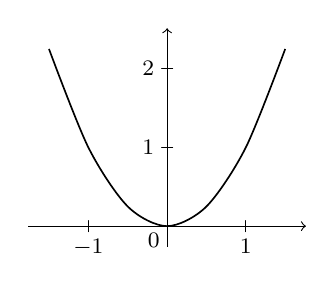
\begin{tikzpicture}
  \datavisualization [school book axes, visualize as smooth line]
    data {
      x, y
      -1.5, 2.25
      -1, 1
      -.5, .25
      0, 0
      .5, .25
      1, 1
      1.5, 2.25
    };
\end{tikzpicture}
\end{codeexample}

\begin{codeexample}[]
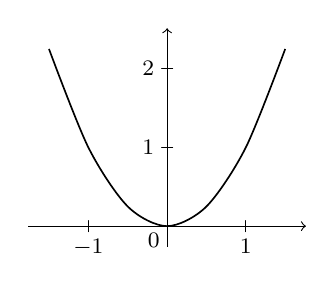
\begin{tikzpicture}
  \datavisualization [school book axes, visualize as smooth line]
    data [format=function] {
      var x : interval [-1.5:1.5] samples 7;
      func y = \value x*\value x;
    };
\end{tikzpicture}
\end{codeexample}

In the first example, no format needed to be specified explicitly since the
default format is the one used for the data following the |data| keyword: A
list of comma-separated values, where each line represents a data point.

\medskip
\textbf{Number accuracy.}\label{section-dv-expressions}
Data visualizations typically demand a much higher accuracy and range of values
than \TeX\ provides: \TeX\ numbers are limited to 13 bits for the integer part
and 16 bits for the fractional part. Because of this, the data visualization
engine does not use \pgfname's standard representation of numbers and \TeX\
dimensions and is does not use the standard parser when reading numbers in a
data point. Instead, the |fpu| library, described in
Section~\ref{section-library-fpu}, is used to handle numbers.

This use of the |fpu| library has several effects that users of the data
visualization system should be aware of:
%
\begin{enumerate}
    \item You can use numbers like |100000000000000| or |0.00000000001| in a
        data points.
    \item Since the |fpu| library does not support advanced parsing, you
        currently \emph{cannot} write things like |3+2| in a data point number.
        This will result in an error.
    \item However, there is a loop-hole: If a ``number'' in a data point starts
        with a parenthesis, the value between the parentheses \emph{is} parsed
        using the normal parser:
        %
        \begin{itemize}
            \item |100000| is allowed.
            \item |2+3| yields an error.
            \item |(2+3)| is allowed and evaluates to |5|.
            \item |(100000)| yields an error since $100\,000$ is beyond the
                normal parser's precision.
        \end{itemize}
        %
        The bottom line is that any normal calculations should be set inside
        round parentheses, while large numbers should not be surrounded by
        parentheses. Hopefully, in the future, these restrictions will be
        lifted.
\end{enumerate}

Section~\ref{section-dv-formats} gives an in-depth coverage of the available
data formats and explains how new data formats can be defined.


\subsection{Concept: Axes, Ticks, and Grids}

Most plots have two or three axes: A horizontal axis usually called the
$x$-axis, a vertical axis called the $y$-axis, and possibly some axis pointing
in a sloped direction called the $z$-axis. Axes are usually drawn as lines with
\emph{ticks} indicating interesting positions on the axes. The data
visualization engine gives you detailed control over where these ticks are
rendered and how many of them are used. Great care is taken to ensure that the
position of ticks are chosen well by default.

From the point of view of the data visualization engine, axes are a somewhat
more general concept than ``just'' lines that point ``along'' some dimension:
The data visualization engine uses axes to visualize any change of an attribute
by varying the position of data points in the plane. For instance, in a polar
plot, there is an ``axis'' for the angle and another ``axis'' for the distance
if the point from the center. Clearly these axes vary the position of data
points in the plane according to some attribute of the data points; but just as
clearly they do not point in any ``direction''.

A great benefit of this approach is that the powerful methods for specifying
and automatic inference of ``good'' positions for ticks or grid lines apply to
all sorts of situations. For instance, you can use it to automatically put
ticks and grid lines at well-chosen angles of a polar plot.

Typically, you will not need to specify axes explicitly. Rather, predefined
styles take care of this for you:
%
\begin{codeexample}[]
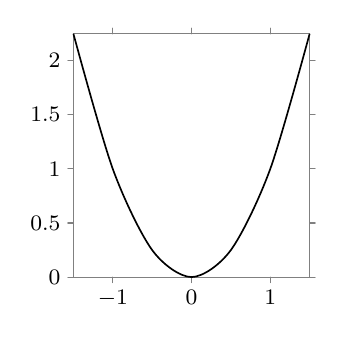
\begin{tikzpicture}
  \datavisualization [
    scientific axes,
    x axis={length=3cm, ticks=few},
    visualize as smooth line
  ]
    data [format=function] {
      var x : interval [-1.5:1.5] samples 7;
      func y = \value x*\value x;
    };
\end{tikzpicture}
\end{codeexample}

\begin{codeexample}[]
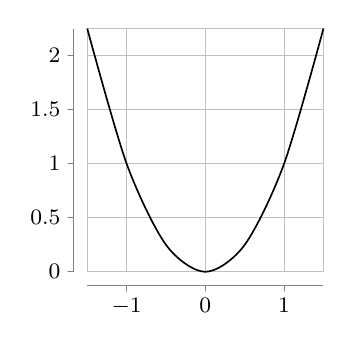
\begin{tikzpicture}
  \datavisualization [
    scientific axes=clean,
    x axis={length=3cm, ticks=few},
    all axes={grid},
    visualize as smooth line
  ]
    data [format=function] {
      var x : interval [-1.5:1.5] samples 7;
      func y = \value x*\value x;
    };
\end{tikzpicture}
\end{codeexample}

Section~\ref{section-dv-axes} explains in more detail how axes, ticks, and grid
lines can be chosen and configured.


\subsection{Concept: Visualizers}

Data points and axes specify \emph{what} is visualized and \emph{where}. A
\emph{visualizer} specifies \emph{how} they are visualized. One of the most
common visualizers is a \emph{line visualizer} which connects the positions of
the data points in the plane using a line. Another common visualizer is the
\emph{scatter plot visualizer} where small marks are drawn at the positions of
the data points. More advanced visualizers include, say, box plot visualizers
or pie chart visualizers.
%
\begin{codeexample}[]
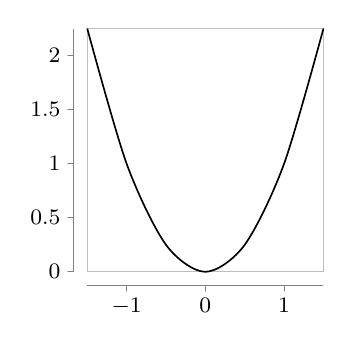
\begin{tikzpicture}
  \datavisualization [
    scientific axes=clean,
    x axis={length=3cm, ticks=few},
    visualize as smooth line
  ]
    data [format=function] {
      var x : interval [-1.5:1.5] samples 7;
      func y = \value x*\value x;
    };
\end{tikzpicture}
\end{codeexample}
%
\begin{codeexample}[]
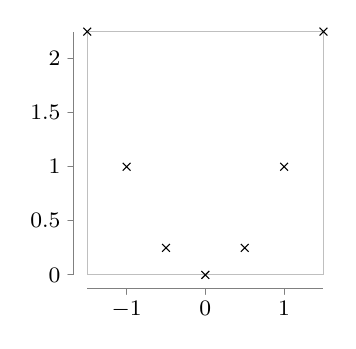
\begin{tikzpicture}
  \datavisualization [
    scientific axes=clean,
    x axis={length=3cm, ticks=few},
    visualize as scatter
  ]
    data [format=function] {
      var x : interval [-1.5:1.5] samples 7;
      func y = \value x*\value x;
    };
\end{tikzpicture}
\end{codeexample}

Section~\ref{section-dv-visualizers} provides more information on visualizers
as well as reference lists.


\subsection{Concept: Style Sheets and Legends}

A single data visualizations may use more than one visualizer. For instance, if
you wish to create a plot containing several lines, a separate visualizer is
used for each line. In this case, two problems arise:
%
\begin{enumerate}
    \item You may wish to make it easy for the reader to differentiate between
        the different visualizers. For instance, one line should be black,
        another should be red, and another blue. Alternatively, you might wish
        one line to be solid, another to be dashed, and a third to be dotted.

        Specifying such styles is trickier than one might expect; experience
        shows that many plots use ill-chosen and inconsistent styling. For this
        reason, the data visualization introduces the notion of \emph{style
        sheets} for visualizers and comes with some well-designed predefined
        style sheets.
    \item You may wish to add information concerning what the different
        visualizers represent. This is typically done using a legend, but it is
        even better to add labels directly inside the visualization. Both
        approaches are supported.
\end{enumerate}

An example where three functions are plotted and a legend is added is shown
below. Two style sheets are used so that \emph{both} the coloring and the
dashing is varied.
%
\begin{codeexample}[]
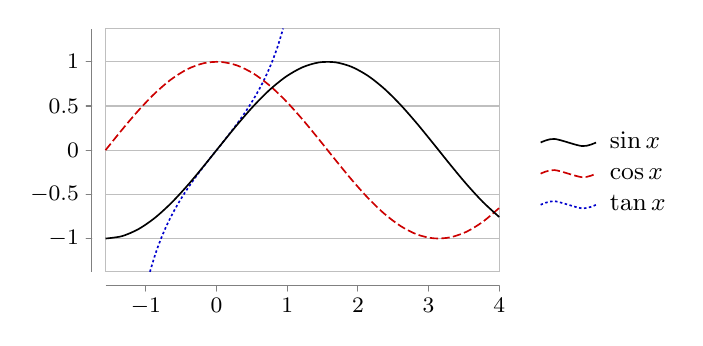
\begin{tikzpicture}[baseline]
  \datavisualization [ scientific axes=clean,
                       y axis=grid,
                       visualize as smooth line/.list={sin,cos,tan},
                       style sheet=strong colors,
                       style sheet=vary dashing,
                       sin={label in legend={text=$\sin x$}},
                       cos={label in legend={text=$\cos x$}},
                       tan={label in legend={text=$\tan x$}},
                       data/format=function ]
  data [set=sin] {
    var x : interval [-0.5*pi:4];
    func y = sin(\value x r);
  }
  data [set=cos] {
    var x : interval [-0.5*pi:4];
    func y = cos(\value x r);
  }
  data [set=tan] {
    var x : interval [-0.3*pi:.3*pi];
    func y = tan(\value x r);
  };
\end{tikzpicture}
\end{codeexample}

Section~\ref{section-dv-style-sheets} details style sheets and legends.


\subsection{Usage}
\label{section-dv-data-syntax}

Inside a \tikzname\ picture you can use the |\datavisualization| command to
create a data visualization. You can use this command several times in a
picture to create pictures containing multiple data visualizations.

\begin{command}{\datavisualization\opt{\oarg{data visualization options}}\meta{data specification}|;|}
    This command is available only inside a |{tikzpicture}| environment.

    The \meta{data visualization options} are used to configure the data
    visualization, that is, how the data is to be depicted. The options are
    executed with the path prefix |/tikz/data visualization|. This means that
    normal \tikzname\ options like |thin| or |red| cannot be used here. Rather,
    a large number of options specific to data visualizations are available.

    As a minimum, you should specify at least two options: First, you should
    use an option that selects an axis system that is appropriate for your
    plot. Typical possible keys are |school book axes| or |scientific axes|,
    detailed information on them can be found in Section~\ref{section-dv-axes}.

    Second, you use an option to select \emph{how} the data should be
    visualized. This is done using a key like |visualize as line| which will,
    as the name suggests, visualize the data by connecting data points in the
    plane using a line. Similarly, |visualize as smooth cycle| will try to fit
    a smooth cycle through the data points. Detailed information on possible
    visualizers can be found in Section~\ref{section-dv-visualizers}.

    Following these options, the \meta{data specification} is used to provide
    the actual to-be-visualized data. The syntax is somewhat similar to
    commands like |\path|: The \meta{data specification} is a sequence of
    keywords followed by local options and parameters, terminated with a
    semicolon. (Indeed, like for the |\path| command, the \meta{data
    visualizers options} need not be specified at the beginning, but additional
    option surrounded by square brackets may be given anywhere inside the
    \meta{data specification}.)

    The different possible keywords inside the \meta{data specification} are
    explained in the following.
\end{command}

\begin{datavisualizationoperation}{data}{\opt{\oarg{options}}\opt{\marg{inline data}}}
    This command is used to specify data for the data visualization. It can be
    used several times inside a single visualization and each time the
    to-be-read data may have a different format, but the data will be
    visualized as if it have been specified inside a single |data| command.

    The behaviour of the |data| command depends on whether the \meta{inline
    data} is present. If it is not present, the \meta{options} must be used to
    specify a source file from which the data is read; if the \meta{inline
    data} is present no file will be used, instead the data should directly
    reside inside the \TeX-file and be given between the curly braces
    surrounding the \meta{inline data}.

    The \meta{options} are executed with the prefix |/pgf/data|. The following
    options are always available:
    %
    \begin{key}{/pgf/data/read from file=\meta{filename} (initially \normalfont empty)}
        If you set the |source| attribute to a non-empty \meta{filename}, the
        data will be read from this file. In this case, no \meta{inline data}
        may be present, not even empty curly braces should be provided.
        %
\begin{codeexample}[code only]
\datavisualization ...
  data [read from file=file1.csv]
  data [read from file=file2.csv];
\end{codeexample}
        %
        The other way round, if |read from file| is empty, the  data must
        directly follow as \meta{inline data}.
        %
\begin{codeexample}[code only]
\datavisualization ...
  data {
    x, y
    1, 2
    2, 3
  };
\end{codeexample}
    \end{key}
    %
    The second important key is |format|, which is used to specify the data
    format:
    %
    \begin{key}{/pgf/data/format=\meta{format} (initially table)}
        Use this key to locally set the format used for parsing the data, see
        Section~\ref{section-dv-formats} for a list of predefined formats.

        The default format is the |table|-format, also known as
        ``comma-separated values''. The first line contains names of attributes
        separated by commas, all following lines constitute a data point where
        the attributes are given by the comma-separated values in that line.
    \end{key}


    \medskip
    \textbf{Presetting attributes.}
    Normally, the inline data or the external data contains for each data point
    the values of the different attributes. However, sometimes you may also
    wish to set an attribute to a fixed value for all data points of a data
    set. Suppose, for instance, that you have to source files
    |experiment007.csv| and |experiment023.csv| and you would like that for all
    data points of the first file the attribute |/data point/experiment id| is
    set to 7 while for the data points of the second file they are set to 23.
    In this case, you can specify the desired settings using an absolute path
    inside the \meta{options}. The effect will be local to the current |data|
    command:
    %
\begin{codeexample}[code only]
\datavisualization...
  data [/data point/experiment=7,  read from file=experiment007.csv]
  data [/data point/experiment=23, read from file=experiment023.csv];
\end{codeexample}

\begin{codeexample}[]
\tikz
  \datavisualization [school book axes, visualize as line]
    data [/data point/x=1] {
      y
      1
      2
    }
    data [/data point/x=2] {
      y
      2
      0.5
    };
\end{codeexample}


    \medskip
    \textbf{Setting options for multiple |data| commands.}
    You may wish to generally set the format once and for all. This can be done
    by using the following key:
    %
    \begin{stylekey}{/tikz/every data}
        This key is executed for every |data| command.
    \end{stylekey}

    Another way of passing options to multiple |data| commands is to use the
    following facility: Whenever an option with the path
    |/tikz/data visualization/data| is used, the path will be remapped to
    |/pgf/data|. This means, in particular, that you can pass an option like
    |data/format=table| to the |\datavisualization| command to set the data
    format for all |data| commands of the data visualization.


    \medskip
    \textbf{Parsing inline data.}
    When you specify data inline, \TeX\ needs to read the data
    ``line-by-line'', while \TeX\ normally largely ignores end-of-line
    characters. For this reason, the data visualization system temporarily
    changes the meaning of the end-of-line character. This is only possible if
    \TeX\ has not already processed the data in some other way (namely as the
    parameter to some macro).

    The bottom line is that you cannot use inline data when the whole
    |\datavisualization| command is passed as a parameter to some macro that is
    not setup to handle ``fragile'' code. For instance, in a \textsc{beamer}
    |frame| you need to add the |fragile| option when a data visualization
    contains inline data.

    The problem does not arise when an external data |source| is specified.
\end{datavisualizationoperation}

\begin{datavisualizationoperation}{data point}{\opt{\oarg{options}}}
    This command is used to specify data a single data point. The
    \meta{options} are simply executed with the path |/data point| and then a
    data point is created. This means that inside the \meta{options} you just
    specify the values of all attributes in key--value syntax.
    %
\begin{codeexample}[]
\tikz \datavisualization [school book axes, visualize as line]
  data point [x=1, y=1]    data point [x=1, y=2]
  data point [x=2, y=2]    data point [x=2, y=0.5];
\end{codeexample}
    %
\end{datavisualizationoperation}

\begin{key}{/tikz/data visualization/data point=\meta{options}}
    This key is the ``key version'' of the previous command. The difference is
    that this key can be used internally inside styles.
    %
\begin{codeexample}[]
\tikzdatavisualizationset{
  horizontal/.style={
    data point={x=#1, y=1}, data point={x=#1, y=2}},
}
\tikz \datavisualization
[ school book axes, visualize as line,
  horizontal=1,
  horizontal=2 ];
\end{codeexample}
    %
\end{key}

\begin{datavisualizationoperation}{data group}{\opt{\oarg{options}}\marg{name}\opt{|+=|\marg{data specifications}}}
    You can store a whole \meta{data specification} in a \emph{data group}.
    This allows you to reuse data in multiple places without having to write
    the data to an external file.

    The syntax of this command comes in the following three variants:
    %
    \begin{itemize}
        \item |data group| \opt{\oarg{options}} \marg{name} |=| \marg{data
            specifications}
        \item |data group| \opt{\oarg{options}} \marg{name} |+=| \marg{data
            specifications}
        \item |data group| \opt{\oarg{options}} \marg{name}
    \end{itemize}
    %
    In the first case, a new data group called \meta{name} is created (an
    existing data group of the same name will be erased) and the following
    \meta{data specifications} is stored in this data group. The data group
    will not be fed to the rendering pipeline, but it is parsed at this point
    as if it were. The defined data group is defined globally, so you can used
    it in subsequent visualizations. The \meta{options} are saved with the
    parsed \meta{data specifications}.

    In the second case, an already existing data group is extended by adding
    the \meta{data specifications} to it.

    In the third case (detected by noting that the \meta{name} is neither
    followed by an equal sign nor a plus sign), the contents of the previously
    defined data group \meta{name} is inserted. The \meta{options} are also
    executed.

    Let is now first create a data group. Note that nothing is drawn since the
    ``dummy'' data visualization is empty and used only for the definition of
    the data group.
    %
\begin{codeexample}[]
\tikz \datavisualization data group {points} = {
  data {
    x, y
    0, 1
    1, 2
    2, 2
    5, 1
    2, 0
    1, 1
  }
};
\end{codeexample}

    We can now use this data in different plots:
    %
\begin{codeexample}[]
\tikz \datavisualization [school book axes,      visualize as line] data group {points};
\qquad
\tikz \datavisualization [scientific axes=clean, visualize as line] data group {points};
\end{codeexample}
    %
\end{datavisualizationoperation}

\begin{datavisualizationoperation}{scope}{\opt{\oarg{options}}\marg{data specification}}
    Scopes can be used to nest hierarchical data sets. The \meta{options} will
    be executed with the path |/pgf/data| and will only apply to the data sets
    specified inside the \meta{data specification}, which may contain |data| or
    |scope| commands once more:
    %
\begin{codeexample}[code only]
\datavisualization...
  scope [/data point/experiment=7]
  {
    data [read from file=experiment007-part1.csv]
    data [read from file=experiment007-part2.csv]
    data [read from file=experiment007-part3.csv]
  }
  scope [/data point/experiment=23, format=foo]
  {
    data [read from file=experiment023-part1.foo]
    data [read from file=experiment023-part2.foo]
  };
\end{codeexample}
    %
\end{datavisualizationoperation}

\begin{datavisualizationoperation}{info}{\opt{\oarg{options}}\marg{code}}
    This command will execute normal \tikzname\ \meta{code} at the end of a
    data visualization. The \meta{options} are executed with the normal path
    |/tikz/|.

    The only difference between this command and just giving the \meta{code}
    directly following the data visualization is that inside the \meta{code}
    following an |info| command you still have access to the coordinate system
    of the data visualization. In sharp contrast, \tikzname\ code given after a
    data visualization can no longer access this coordinate system.
    %
\begin{codeexample}[]
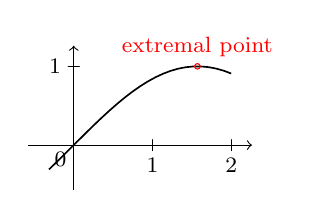
\begin{tikzpicture}[baseline]
  \datavisualization [ school book axes, visualize as line ]
  data [format=function] {
    var x : interval [-0.1*pi:2];
    func y = sin(\value x r);
  }
  info {
    \draw [red] (visualization cs: x={(.5*pi)}, y=1) circle [radius=1pt]
      node [above,font=\footnotesize] {extremal point};
  };
\end{tikzpicture}
\end{codeexample}

    As can be seen, inside a data visualization a special coordinate system is
    available:

    \begin{coordinatesystem}{visualization}
        As for other coordinate systems, the syntax is
        \declare{|(visualization cs:|\meta{list of attribute-value pairs}|)|}.
        The effect is the following: For each pair
        \meta{attribute}|=|\meta{value} in the \meta{list} the key
        |/data point/|\meta{attribute} is set to \meta{value}. Then, it is
        computed where the resulting data point ``would lie'' on the canvas
        (however, no data point is passed to the visualizers).
    \end{coordinatesystem}
\end{datavisualizationoperation}

\begin{datavisualizationoperation}{info'}{\opt{\oarg{options}}\marg{code}}
    This command works like |info|, only the \meta{code} will be executed just
    before the visualization is done. This allows you to draw things
    \emph{behind} the visualization.
    %
\begin{codeexample}[]
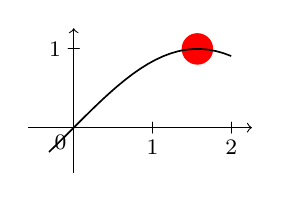
\begin{tikzpicture}[baseline]
  \datavisualization [ school book axes, visualize as line ]
  data [format=function] {
    var x : interval [-0.1*pi:2];
    func y = sin(\value x r);
  }
  info' {
    \fill [red] (visualization cs: x={(.5*pi)}, y=1) circle [radius=2mm];
  };
\end{tikzpicture}
\end{codeexample}
    %
\end{datavisualizationoperation}

\label{section-dv-bounding-box}%
\begin{predefinednode}{data visualization bounding box}
    This rectangle node stores a bounding box of the data visualization that is
    currently being constructed. This node can be useful inside |info| commands
    or when labels need to be added.
\end{predefinednode}

\begin{predefinednode}{data bounding box}
    This rectangle node is similar to |data visualization bounding box|, but it
    keeps track only of the actual data. The spaces needed for grid lines,
    ticks, axis labels, tick labels, and other all other information that is
    not part of the actual data is not part of this box.
\end{predefinednode}


\subsection{Advanced: Executing User Code During a Data Visualization}
\label{section-dv-user-code}

The following keys can be passed to the |\datavisualization| command and allow
you to execute some code at some special time during the data visualization
process. For details of the process and on which signals are emitted when, see
Section~\ref{section-dv-backend}.

\begin{key}{/tikz/data visualization/before survey=\meta{code}}
    The \meta{code} is passed to the |before survey| method of the data
    visualization object and then executed at the appropriate time (see
    Section~\ref{section-dv-backend} for details).

    The following commands work likewise:
\end{key}
%
\begin{key}{/tikz/data visualization/at start survey=\meta{code}}
\end{key}
%
\begin{key}{/tikz/data visualization/at end survey=\meta{code}}
\end{key}
%
\begin{key}{/tikz/data visualization/after survey=\meta{code}}
\end{key}
%
\begin{key}{/tikz/data visualization/before visualization=\meta{code}}
\end{key}
%
\begin{key}{/tikz/data visualization/at start visualization=\meta{code}}
\end{key}
%
\begin{key}{/tikz/data visualization/at end visualization=\meta{code}}
\end{key}
%
\begin{key}{/tikz/data visualization/after visualization=\meta{code}}
\end{key}


\subsection{Advanced: Creating New Objects}

You will need the following key only when you wish to create new rendering
pipelines from scratch -- instead of modifying an existing pipeline as you
would normally do. In the following it is assumed that you are familiar with
the concepts of Section~\ref{section-dv-backend}.

\begin{key}{/tikz/data visualization/new object=\meta{options}}
    This key serves two purposes:
    %
    \begin{enumerate}
        \item This method makes it easy to create a new object as part of the
            rendering pipeline, using \meta{options} to specify arguments
            rather that directly calling |\pgfoonew|. Since you have the full
            power of the keys mechanism at your disposal, it is easy, for
            instance, to control whether or not parameters to the constructor
            are expanded or not.
        \item The object is not created immediately, but only just before the
            visualization starts. This allows you to specify that an object
            must be created, but the parameter values of for its constructor
            may depend on keys that are not yet set. A typical application is
            the creating of an axis object: When you say |scientific axes|, the
            |new object| command is used internally to create two objects
            representing these axes. However, keys like |x={length=5cm}| can
            only \emph{later} be used to specify the parameters that need to be
            passed to the constructor of the objects.
  \end{enumerate}

    The following keys may be used inside the \meta{options}:
    %
    \begin{key}{/tikz/data visualization/class=\meta{class name}}
        The class of the to-be-created object.
    \end{key}
    %
    \begin{key}{/tikz/data visualization/when=\meta{phase name} (initially before survey)}
        This key is used to specify when the object is to be created. As
        described above, the object is not created immediately, but at some
        time during the rendering process. You can specify any of the phases
        defined by the data visualization object, see
        Section~\ref{section-dv-backend} for details.
    \end{key}
    %
    \begin{key}{/tikz/data visualization/store=\meta{key name}}
        If the \meta{key name} is not empty, once the object has been created,
        a handle to the object will be stored in \meta{key name}. If a handle
        is already stored in \meta{key name}, the object is not created twice.
    \end{key}
    %
    \begin{key}{/tikz/data visualization/before creation=\meta{code}}
        This code is executed right before the object is finally created. It
        can be used to compute values that are then passed to the constructor.
    \end{key}
    %
    \begin{key}{/tikz/data visualization/after creation=\meta{code}}
        This code is executed right after the object has just been created. A
        handle to the just-created object is available in |\tikzdvobj|.
    \end{key}
    %
    \begin{key}{/tikz/data visualization/arg1=\meta{value}}
        The value to be passed as the first parameter to the constructor.
        Similarly, the keys |arg2| to |arg8| specify further parameters passed.
        Naturally, only as many arguments are passed as parameters are set.
        Here is an example:
        %
\begin{codeexample}[code only]
\tikzdatavisualizationset{
  new object={
    class = example class,
    arg1  = foo,
    arg2  = \bar
  }
}
\end{codeexample}
        %
        causes the following object creation code to be executed later on:
        %
\begin{codeexample}[code only]
\pgfoonew \tikzdvobj=new example class(foo,\bar)
\end{codeexample}
        %
        Note that you key mechanisms like |.expand once| to pass the value of a
        macro instead of the macro itself:
        %
\begin{codeexample}[code only]
\tikzdatavisualizationset{
  new object={
    class              = example class,
    arg1               = foo,
    arg2/.expand once  = \bar
  }
}
\end{codeexample}
        %
        Now, if |\bar| is set to |This \emph{is} it.|\@ at the moment to object
        is created later on, the following object creation code is executed:
        %
\begin{codeexample}[code only]
\pgfoonew \tikzdvobj=new example class(foo,This \emph{is} it)
\end{codeexample}
    \end{key}

    \begin{key}{/tikz/data visualization/arg1 from key=\meta{key}}
        Works like the |arg1|, only the value that is passed to the constructor
        is the current value of the specified \meta{key} at the moment when the
        object is created.
        %
\begin{codeexample}[code only]
\tikzdatavisualizationset{
  new object={
    class              = example class,
    arg1 from key      = /tikz/some key
  }
}
\tikzset{some key/.initial=foobar}
\end{codeexample}
        %
        causes the following to be executed:
        %
\begin{codeexample}[code only]
\pgfoonew \tikzdvobj=new example class(foobar)
\end{codeexample}
        %
        Naturally, the keys |arg2 from key| to |arg8 from key| are also
        provided.
    \end{key}

    \begin{key}{/tikz/data visualization/arg1 handle from key=\meta{key}}
        Works like the |arg1 from key|, only the key must store an object and
        instead of the object a handle to the object is passed to the
        constructor.
    \end{key}
\end{key}
